\documentclass[11pt, oneside]{article} 
\usepackage{geometry}
\geometry{letterpaper} 
\usepackage{graphicx}
	
\usepackage{amssymb}
\usepackage{amsmath}
\usepackage{parskip}
\usepackage{color}
\usepackage{hyperref}

\graphicspath{{/Users/telliott_admin/Tex/png/}}
% \begin{center} 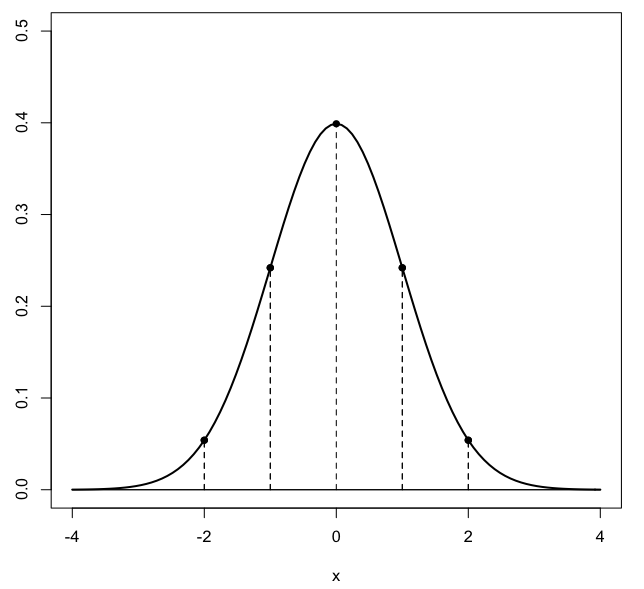
\includegraphics [scale=0.4] {gauss3.png} \end{center}

\title{Sum of angles by similar triangles}
\date{}

\begin{document}
\maketitle
\Large

\subsection*{cosine of a sum}

The sum of angle formulas (i.e. formulas for the sine and cosine of the sum or difference of two angles) are used often in calculus, not only for working problems, but even in the derivation of the "derivative" of sine and cosine.

You really must know them.  I think it's so important that we will show three ways of finding these formulas --- not all in this chapter.  The easiest way to remember them uses Euler's equation, and we won't be ready for that until later.  See \hyperref[sec:Euler_sum_angles]{\textbf{here}}.

There are four equations:  $\sin s \pm t$ and $\cos s \pm t$.

I've memorized only this one:
\[ \cos s - t = \cos s \cos t + \sin s \sin t \]

By $\cos s - t$ we mean $\cos (s - t)$, but have left off the parentheses.  

Say "cos cos" and then recall the difference in sign.

\subsection*{check}

I like this version because it can be checked easily.  Set $s = t$:
\[ \cos s - t = \cos 0 = 1 = \cos^2 s + \sin^2 s \]
which is our favorite trigonometric identity and obviously correct.

\subsection*{change signs}

For $\cos s + t $ flip the sign on the second term.  
\[ \cos s + t = \cos s \cos t - \sin s \sin t \]
This is simply a result of the fact that

\[ \cos -\theta = \cos \theta \]
\[ \sin - \theta = - \sin \theta \]

\begin{center} 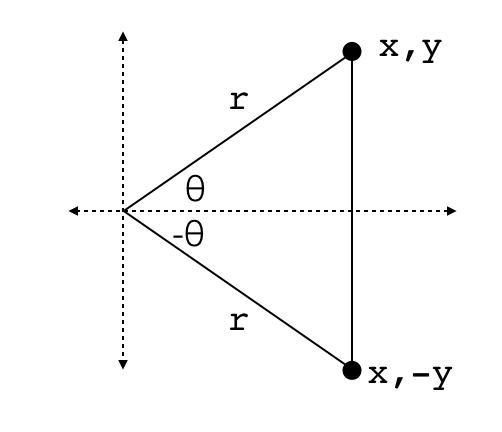
\includegraphics [scale=0.4] {pm_theta.png} \end{center}

The diagram shows the reason:  $\cos \theta = \cos - \theta = x/r$ while $\sin \theta = y/r = -  (\sin - \theta ) = - (-y/r)$.

Proof:
\[ \cos (s - (-u)) = \cos s \cos (-u) + \sin s \sin (-u) \]
Since $\cos -x = \cos x$ and $\sin -x = -\sin x$:
\[ \cos (s + u) = \cos s \cos u - \sin s \sin u \]
But $u$ is just a dummy variable (it could be any symbol), so
\[ \cos (s + t) = \cos s \cos t - \sin s \sin t \]

\subsection*{sine of a sum}
We will look at the proof for the sine formula later, for now just write it:
\[ \sin s + t = \sin s \cos t + \sin t \cos s \]

Say "sin cos" and then, that here $+$ goes with $+$.  Like most things having to do with sine and cosine, there is a change of sign when changing from one to the other.

For $\sin s - t$, flip the sign on the second term, as before.

\subsection*{proof}
Here is a geometric proof of both of the sum of angles formulas, using similar triangles.  The key is to draw an inspired diagram.

Consider a right triangle, with one of the angles labeled $s$.  Construct another right triangle containing angle $t$, and scale it so that the base adjacent to angle $t$ is just as long as the hypotenuse of the triangle containing angle $s$, and draw them one on top of the other as shown:

Scale the joined triangles so that the hypotenuse of the second triangle has unit length.  Our crucial insight is to draw vertical and horizontal dotted lines as shown below.  
\begin{center} 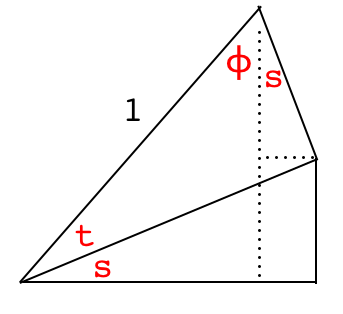
\includegraphics [scale=0.4] {sum_angles1.png} \end{center}

The angle $s$ is part of a right triangle with angle $t$ adjacent, where the third acute angle is $\phi$.  But $\phi$ is also part of a second right angle containing $t$ plus the angle adjacent to $\phi$.  Therefore, that adjacent angle is also equal to angle $s$.

We add some labels to the sides of the triangles and calculate the sine and cosine of $s$, $t$ and $s + t$:
\begin{center} 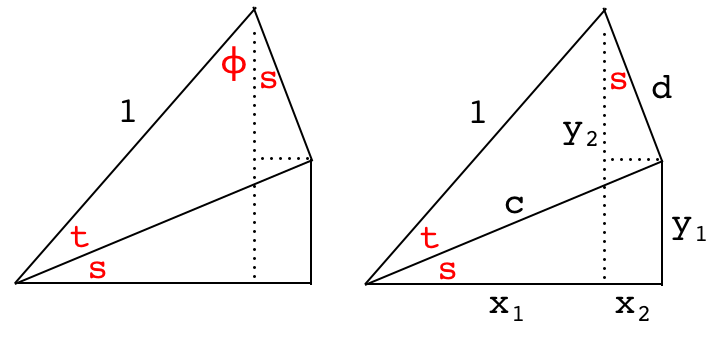
\includegraphics [scale=0.4] {sum_angles2.png} \end{center}
Since I already know the result I am looking for, I write what we had before
\[ \cos s \cos t - \sin s \sin t \]

From the figure
\[ \cos s = \frac{x_1 + x_2}{c}; \ \ \ \cos t = \frac{c}{1}; \ \ \ \cos s \cos t = x_1 + x_2 \]
The sine of $s$ is a little trickier, look at the small right triangle at the top of the figure
\[ \sin s = \frac{x_2}{d}; \ \ \ \sin t = \frac{d}{1}; \ \ \ \sin s \sin t = x_2   \]

The difference is
\[  \cos s \cos t - \sin s \sin t = x_1 \]
but from the diagram it's clear that
\[ \cos s + t = x_1 \]
$\square$

As a quick check we can ask what happens to the formula 
\[ \cos s + t = \cos s \cos t - \sin s \sin t \]
when $t = 0$.  Then the first term is the cosine of $s$, and the second term is equal to $0$.  The formula is symmetrical with respect to $s$ and $t$.

\subsection*{extension to sine}
Referring back to the diagram (and again, with our goal clearly in mind)
\begin{center} 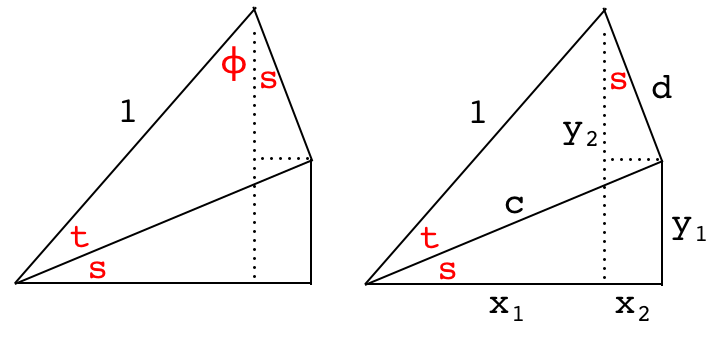
\includegraphics [scale=0.4] {sum_angles2.png} \end{center}

\[ \sin s =  \frac{y_1}{c}; \ \ \ \  \cos t = \frac{c}{1}; \ \ \ \  \sin s \cos t = y_1  \]
\[ \sin t = \frac{d}{1}; \ \ \ \  \cos s = \frac{y_2}{d}; \ \ \ \ \sin t \cos s = y_2 \]
But 
\[ \sin s + t = y_1 + y_2 =  \sin s \cos t +  \sin t \cos s \]

Using the even/odd function rules, we get
\[ \sin s - t = c + d =  \sin s \cos t -  \sin t \cos s \]
And that's all four of them.
\end{document}  